\chapter{Evaluation}
%TODO: Gewichtete Ergebnisse aller Algorithmen-Featuresets-Kombinationen, also Zusammenfassung von basicstats bzw featuresets/all barplots stat boxplot!
%\cite[S.~21]{Demberg2006}: Rule learning: Test=Train

\section{Training}
Das Training der Lernalgorithmen sowie die Klassifizierung je Testset habe ich mit Wekas Knowledge Flow durchgeführt. Die Featuresets habe ich aus den Trainingsdaten generiert, in dem ich alle sonstigen Features herausgefiltert habe. Das Ergebnis der Klassifizierung jedes Testsets ist eine CSV-Datei mit der \enquote{wahren} Klasse und den vorhergesagten Klassen aller Modelle (alle Classifier/Featuresets-Kombinationen).\\
\begin{figure}[h]
    \begin{floatrow}
        \ffigbox{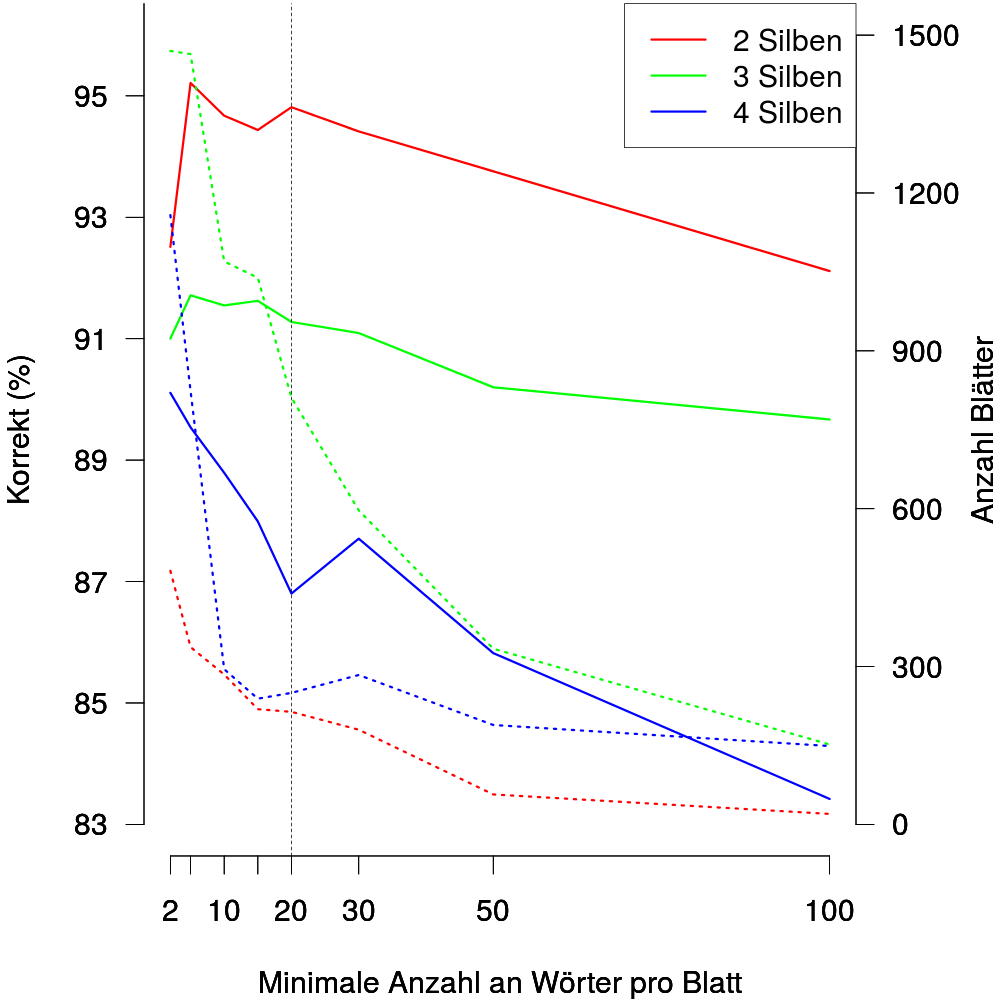
\includegraphics[scale = 0.18]{figures/j48_min_leaves.png}} {
            \label{figure:j48_min_leaves}
            \caption{Einfluss der Anzahl der minimalen Elemente pro Blatt auf die Erkennungsrate (links, fortlaufende Linie) und Breite des Baumes (rechts, gestrichelt). 66\% Training, 33\% Test.}
        }
        \ffigbox{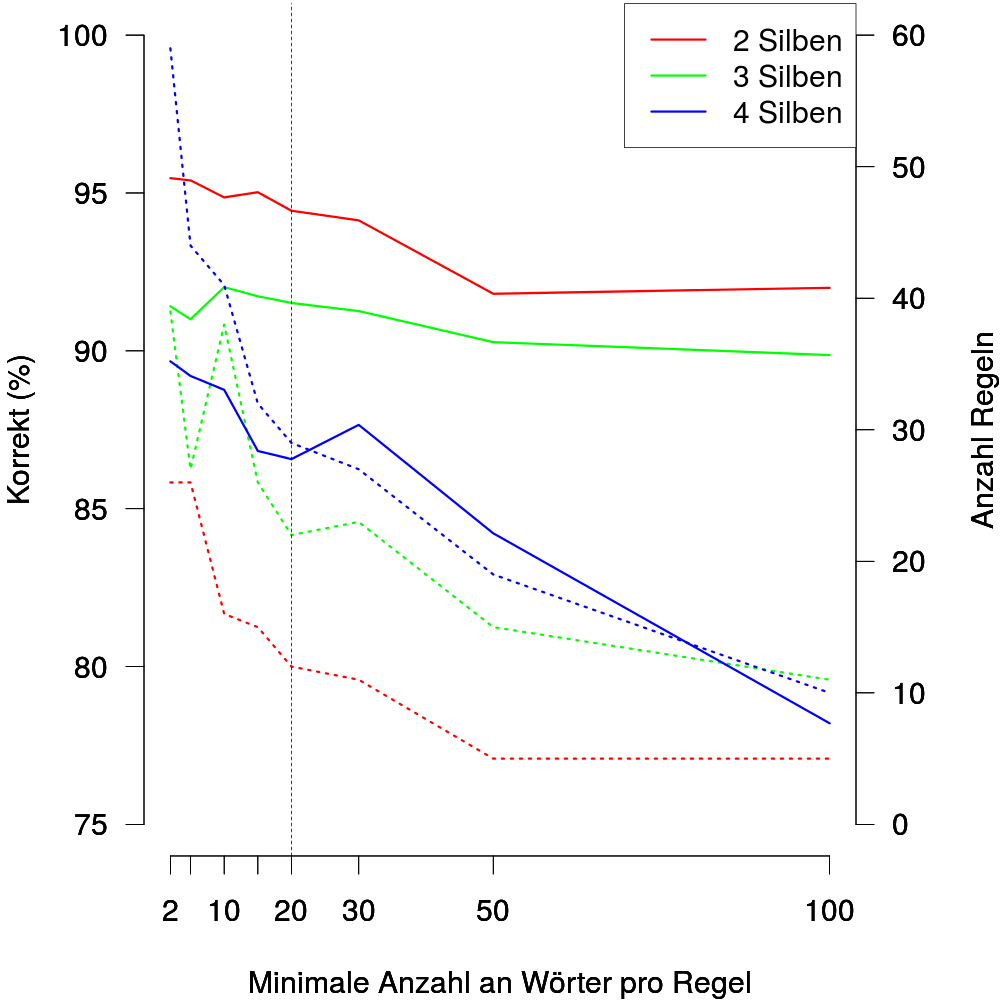
\includegraphics[scale = 0.18]{figures/jrip_min_leaves.png}} {
            \label{figure:jrip_min_leaves}
            \caption{Einfluss der Anzahl der minimalen Elemente pro Regel auf die Erkennungsrate (links, fortlaufende Linie) und Breite des Baumes (rechts, gestrichelt). 66\% Training, 33\% Test.}
        }
    \end{floatrow}
\end{figure}
Beim Training von J48\footnote{Exakte Konfiguration von J48: \texttt{weka.classifiers.trees.J48 -C 0.25 -M 20}} und JRip\footnote{Exakte Konfiguration von JRip: \texttt{weka.classifiers.rules.JRip -F 3 -N 20.0 -O 5 -S 1}} habe ich die minimale Anzahl an Elementen pro Blatt bzw. pro Regel auf 20 limitiert. Durch diese untere Grenze vermeide ich zu spezialisierte Regeln, die nur auf sehr wenige Einzelfälle zutreffen und versuche so irritierendes Rauschen in den Daten auszublenden. Diese Zahl als untere Grenze habe ich empirisch als guten Kompromiss zwischen Kompaktheit und Differenziertheit festgestellt (Abbildung \ref{figure:j48_min_leaves} und \ref{figure:jrip_min_leaves}). Die anderen Parameter habe ich auf ihren Standard-Einstellingen belassen.
Zum Training der Neural Networks habe ich das Modul \textit{NeuralNetwork}\footnote{Verfügbar unter: https://github.com/amten/NeuralNetwork} von Weka verwendet, es bietet Dropout-Regularisierung und RectifiedLinearUnits (ReLUs) als Aktivierungsfunktion. Es ist damit aktuell das modernste und ausgereifteste Neural-Network Modul für Weka. Das Training ist zudem sehr effektiv, kaum eins meiner Modelle hat mehr als 200 Trainingsepochen benötigt, meist reichten ca. 70 Epochen.\\
\begin{figure}[h]
    \centering
    \caption{Ergebnisse der Neuronalen Netze in Abhängigkeit von der Anzahl der Neuronen im Hidden Layer. (66\% Training, 33\% Test)}
    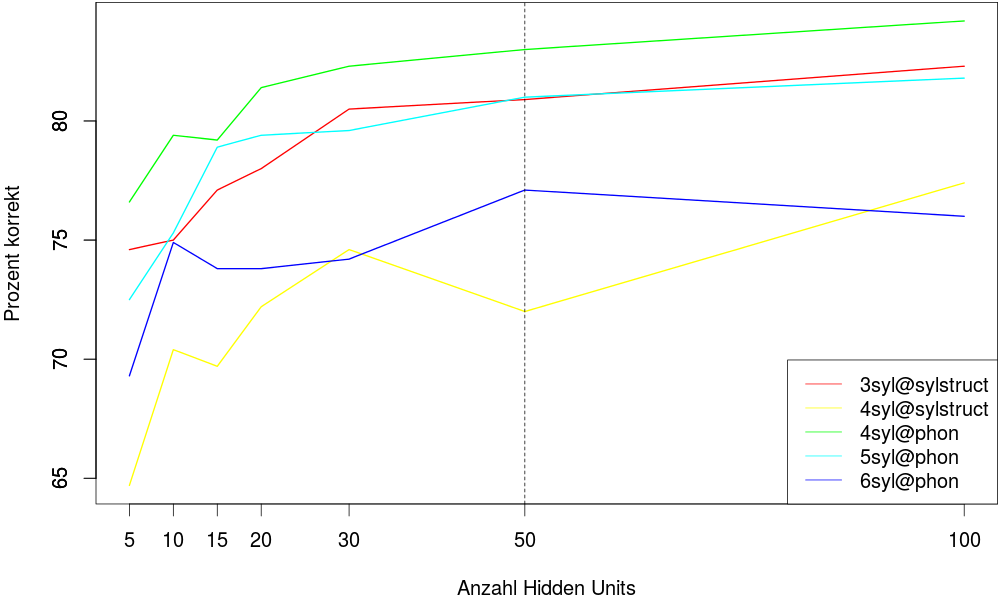
\includegraphics[width=.75\columnwidth]{figures/NN_HUs.png}
    \label{figure:NN_HUs}
\end{figure}
Ich habe eine einschichtige Feed-Forward Architektur mit 50 Hidden Units gewählt\footnote{\label{nn_conf}Exakte Konfiguration des NeuralNetwork: \texttt{weka.classifiers.functions.NeuralNetwork -lr 0.0 -wp 1.0E-8 -mi 1000 -bs 0 -th 4 -hl 50 -di 0.2 -dh 0.5 -iw 0}}. Experimente mit mehr HUs brachten nur geringfügig bessere Ergebnisse (Abbildung \ref{figure:NN_HUs}) und ein weiterer Hidden Layer hat in einzelnen Experimenten auch keine besseren Ergebnisse erzielt. Die längere Trainingszeit und höhere Komplexität des Netzwerks mit mehr Hidden Units wogen für mich schwerer als die geringfügig besseres Ergebnisse. Nach der Regel von \textit{Ockham's razor} sollte man zudem unter gleichwertigen Lösungen die einfachste wählen \cite[S.~652]{RusselNorvig2013}, da Einfachheit an sich eine wünschenswerte Eigenschaft ist, und einfache Modelle besser generalisieren. Obwohl Ockham's razor nicht unumstritten ist \cite{Domingos}, orientiere ich mich in meiner Arbeit an dieser Regel, da einfache Modelle besser verständlich sind und die Gefahr eines Overfittings geringer ist\cite[S.~6]{Domingos}. In meinem Fall bezieht sich Ockham's razor also auf die Architektur des Neural Netowrks mit den wenigsten Neuronen, die Größe des JRip-Regelsets und die Breite des J48-Entscheidungsbaumes.

Als Evaluations-Metrik soll im folgenden die Anzahl an korrekt klassifizierten Wörtern genügen.

\section{Ergebnisse}

Um über die vielen Einzelergebnisse in ihrer Gesamtheit sprechen zu können, ist es notwendig die Ergebnisse sinnvoll zusammenzufassen. Ohne eine entsprechende Aggregation habe ich 6 Datensets (2-7 Silben), 3 Algorithmen (J48, JRip, NeuralNetwork) und 13 Featuresets. Somit gilt es sich einen Überblick über 234 Einzelergebnisse zu verschaffen.

Um die Ergebnisse im Verhältnis zur Schwierigkeit des Problems betrachten zu können stelle ich in jeder Abbildung das Ergebniss des trivialen Baseline-Algorithmus \texttt{ZeroR}, meist als gestrichelte Linie, dar. \texttt{ZeroR} lernt die häufigste Klasse im Trainingsset und klassifiziert alle Wörter des Testsets entsprechend dieser Klasse. Sein Ergebniss stellt somit die \enquote{statistische Nulllinie} dar. Ist ein Algorithmus lediglich so gut wie \texttt{ZeroR}, hat er grob gesagt aus den Features nichts sinnvolles lernen können.

Bei der Betrachtung der folgenden Abbildungen muss man beachten, dass es drei Arten von Featuresets gibt. \texttt{suffix, praefix, sonority, weight, phoncat, meta} sind \textit{grundlegende Featuresets}, die lediglich einen isolierten lingistischen Aspekt betrachten.
Die \textit{kombinierten Featuresets} \texttt{affix} und \texttt{phon} bestehen aus den grundlegenden Featuresets \texttt{praefix} und \texttt{suffix} bzw. \texttt{sonority}, \texttt{weight}, \texttt{phoncat}.
Featureset übergreifende Sammlungen von Einzelfeatures sind die \textit{höheren Featuresets} \texttt{sparse} und \texttt{numeric} während in \texttt{all} sämtliche Features enthalten sind.

Im Folgenden möchte ich zunächst einen Blick auf die Gesamtergebnisse werfen, bei denen die Ergebnisse der einzelnen Modelle nach Trainingssetgröße gewichtet wurden (Abbildung \ref{fig:overall_weighted}). 
% Confusion Matrix => Welche Fehler werden am häufigsten gemacht? Sind seltene Klassen die schwierigen?

\begin{figure}[h]
    \centering
    \caption{Performance je Model, gewichtet über die Trainingssets in Prozent}
    \label{fig:overall_weighted}
    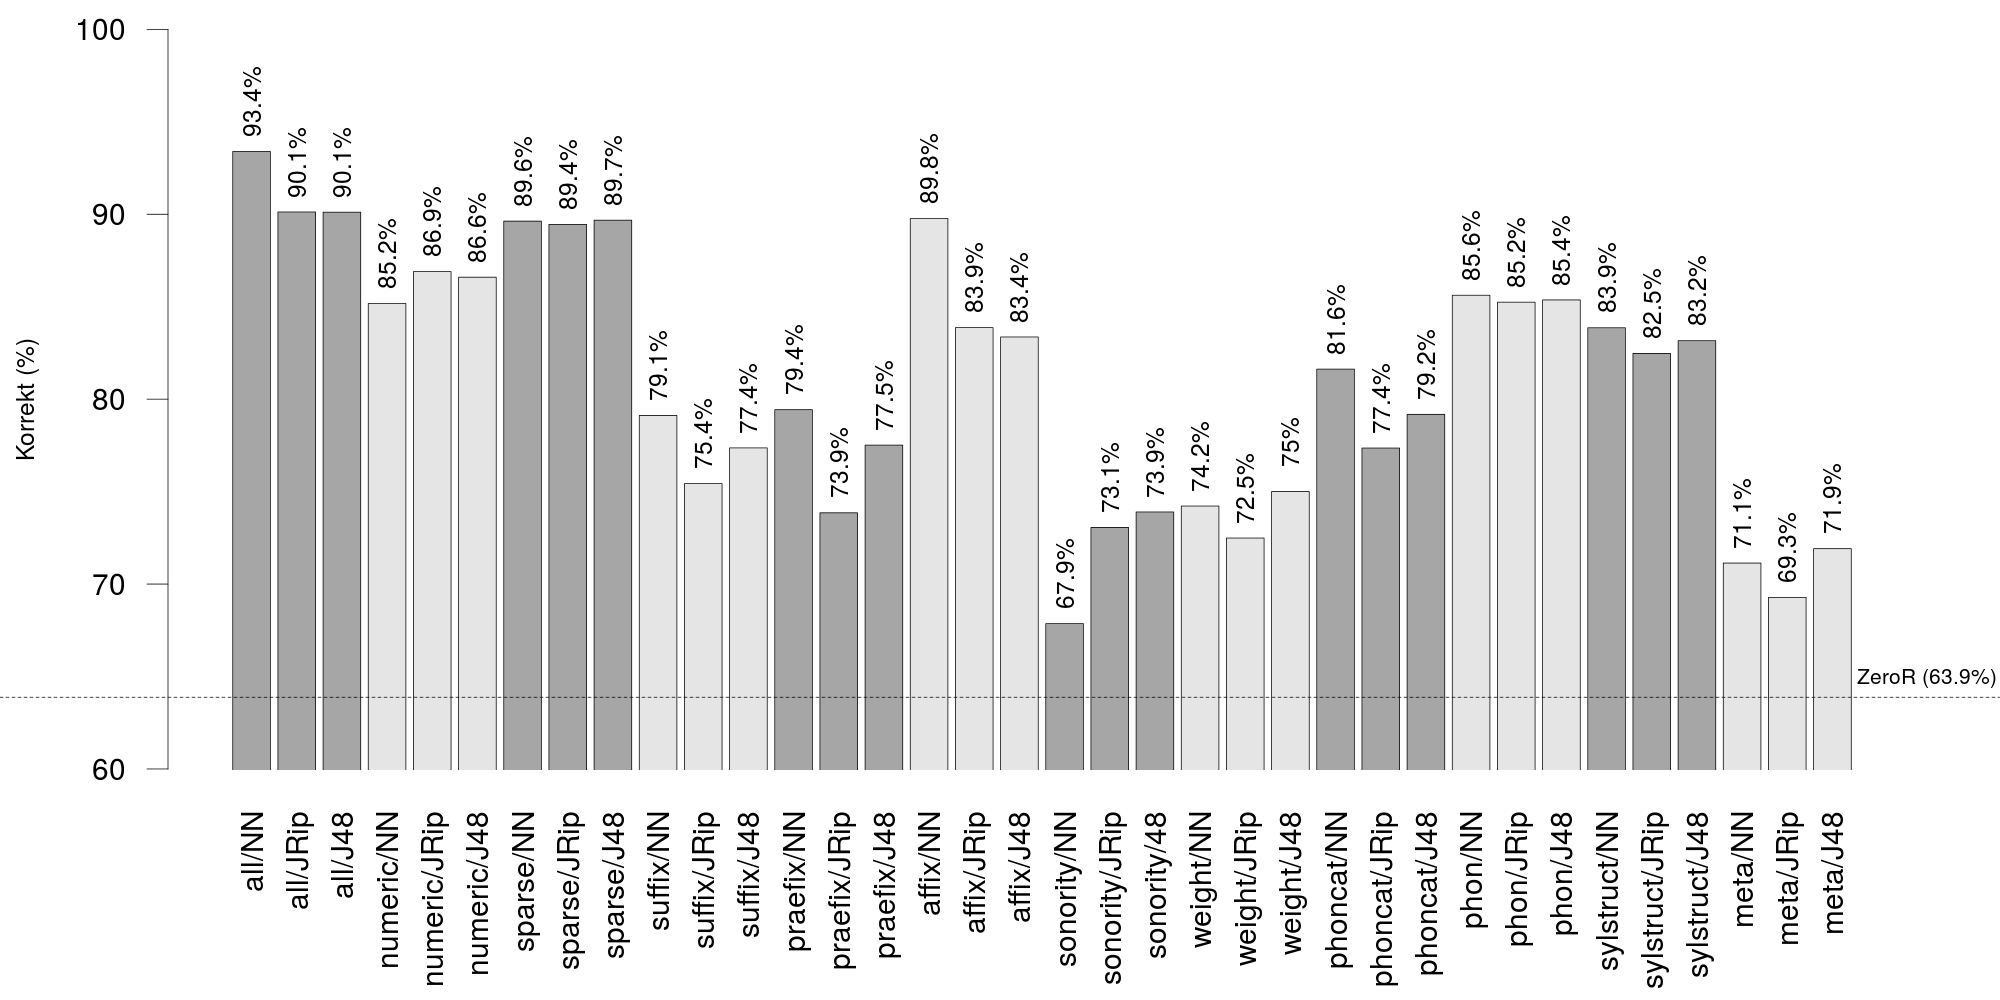
\includegraphics[width=\columnwidth]{figures/esemble/weighted_performance.png}
\end{figure}

Generell kann man der Abbildung \ref{fig:overall_weighted} entnehmen, dass Featuresets mit unterschiedlichen Features besser sind als welche, die nur einzelne linguistische Aspekte betrachten. So sind die Featuresets \texttt{sonority} (67.9-73.9\%), \texttt{weight} (72.5-75.0\%) und \texttt{phonstruct} (77.4-81.6\%) allein eher schwach, in Kombination in \texttt{phon} erreichen alle drei Algorithmen über 85\%. Gleiches trifft auch auf \texttt{praefix} (73.9-79.4\%) und \texttt{suffix} (75.4-79.1\%) sowie ihre Kombination in \texttt{affix} (83.4-89.8\%) zu. Dafür, dass \texttt{sylstruct} ein grundlegendes Featureset ist, erreiche ich mit ihm sehr gute Ergebnisse um die 83\%.  Die drei höheren Featuresets \texttt{all}, \texttt{numeric}, \texttt{sparse} erreichen insgesamt die besten Ergebnisse, angeführt von \texttt{all/NN} mit $93.4\%$. Beste symbolische Modell sind \texttt{all/JRip} und \texttt{all/J48} mit je 90.1\%\\

%Betrachten wir erst die Entscheidungsbäume von J48 hinsichtlich ihrer Varianz. Eine kleine Varianz bedeutet, dass über alle Testsets hinweg ähnliche Erkennungsraten realisiert wurden. Bei kleiner Varianz sind die Features eines Featuresets also unabhängig von der Silbenzahl gleichbedeutend. Sie stellen also Korrelate zum Wortakzent dar, die unabhängig von der Silbenzahl sind, was eine gute Eigenschaft ist. Ist die Varianz groß, ist ein Featureset nicht für alle Silbenanzahlen geeignet, kann jedoch für bestimmten Silbenzahl dennoch gute Ergebnisse liefern. Featuresets mit großer Varianz und guten Ergebnissen sind wahrscheinlich durch Methoden wie Bagging gut anzuwenden.
%Featuresets mit kleiner Varianz und geringen Erkennungsraten sind somit schlecht zur Vorhersage des Akzents geeignet, bei geringer Varianz und hohen Erkennungsraten sind die Features sehr ausdrucksstark. Ist die Varianz groß, werden spezialisiertere Regeln erfasst, die man kombinieren sollte.
%Große Varianz weisen die Affix-Featuresets praefix, suffix und affix auf, ihr Median ist zudem recht gering. Gleiches zeigt sich bei diesem Featuresets bei JRip, insbesondere bei nach unten gibt es starke Ausreißer. Durch die Bediengung, dass jedes Blatt/jede Regel mindestens 20 Elemente enthalten muss fällt es diesen Algorithmen mit abnehmenden Trainingsset-Umfang zunehmend schwerer diese zu berücksichtigen, da die meisten Features dieser Featuresets sehr viele verschiedene Werte enthalten (siehe Tabelle \ref{table:feature_dimensions}). Bemerkenswert sind jedoch die konstant sehr hohen Erkennungsraten von affix/NN. Bei Zwei- bis Viersilbern liefert dieses Modell kurz hinter all/NN die besten Ergebnisse (Detailierte Erkennungsraten siehe Anhang \ref{performance_details}). sonority/NN hingegen ist bei Zweisilbern jedoch nicht besser als ZeroR, wahrscheinlich war die learning rate zu hoch, so dass lediglich die häufigste Klasse gelernt wurde.

\begin{figure}[h]
    \centering
    \caption{Nach Testsetgröße gewichtete Ergebnisse simpler Esembles aus den besten Algorithmen je Feature und Testset. Verbesserung im Vergleich zu Abbildung \ref{fig:overall_weighted} ist grün hervorgehoben.}
    \label{fig:overall_bag}
    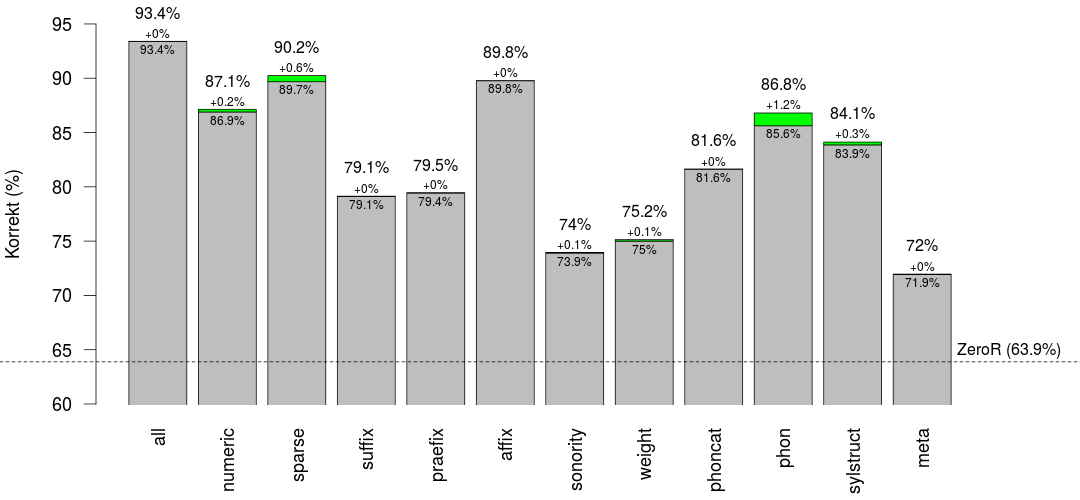
\includegraphics[width=.85\columnwidth]{figures/esemble/bag_of_best_algorithms_for_featuresets.png}
\end{figure}

In Abbildung \ref{fig:overall_bag} sind die Ergebnisse eines simplen Esembles zu sehen, das aus den jeweils besten Modellen der sechs Testsets besteht. Für jedes Testset habe ich je Featureset das beste Modell (J48, JRip oder NN) ausgewählt. Im Falle des phon-Esembles, bestehend aus phon/J48 für Zwei- und Dreisilber und phon/NN für Wörter mit mehr Silben, wird eine Verbesseurng um 1.2\% erreicht. Wahrscheinlich lassen sich die Ergebnisse durch komplexere Esemble-Techniken wie Bagging \cite{Breiman1996} weiter verbessern. Für effektive Anwendung von Esemble-Techniken ist es wichtig, dass die verschiedenen Modelle möglichst wenig korreliert sind, da sie sonst häufiger die gleiche Vermutung für die Klassifizierung abgeben und das Esemble recht sinnlos wäre. Da die Featuresets zum Teil komplett verschiedene linguistische Aspekte betrachten ist anzunehmen, dass sie ausreichend wenig korreliert sind um in Esembles gut verwendet werden zu können. Dies jedoch nur am Rande. Durch Bagging gibt man jedoch die Interpretierbarkeit zugunsten einer höheren Genauigkeit auf \cite[S.\~137]{Breiman1996}, weswegen ich hier diesen Ansatz nicht weiter verfolgen werde.